\documentclass[a4paper,UKenglish]{lipics-v2018}
\usepackage{microtype}%if unwanted, comment out or use option "draft"
\bibliographystyle{plainurl}

\title{Formal Methods for Security - Final Report}

\author{Daniel Schaefer}{2549458}{}{}{}
\authorrunning{Daniel Schaefer}
\renewcommand{\copyrightline}{}

\def\murphi{Mur$\phi$ }

\begin{document}
\maketitle

\begin{abstract}


The design of security protocols is a notoriously error-prone task and unfortunately, those errors can not be detected by functional testing, since they appear only in the presence of a malicious adversary. It is quite obvious that proving security properties of protocols is very valuable, especially if we do not have to make very strict assumptions doing so.

In this course we generally talked about various formal methods of verifying security of software or protocols. The papers that were part of the reading session build a basis regarding model-checking in this field and a commonly occurring approach of self-composition, which can be used to verify secure information flow of some program. On the other hand, \murphi as a prime example of classic forward state-exploration.

The main problem of the model-checking approach is the state-space explosion problem, which gets introduced by the infinite number of sessions that the non-deterministic adversary is able to interact with. One way to overcome this issue is by 'redirecting' it to the user of the verifier, who inputs upper bounds for e.g. the number of sessions that are executed in parallel. While this makes the state-space finite, it clearly also weakens the security proof as there might be an attack which requires more sessions than the bound was set to.

A different approach is taken by tools such as \textit{ProVerif}, which abstracts much further away from the protocol executions, by building an alternative representation of the protocol which intuitively combines the protocol with the attacker already. While this does not guarantee termination, as the state-space is still infinite, it terminates most of the time in practice and requires much less human-intervention which obviously decreases the risk of \textit{human error}.

Information flow verification also turned out to be a prominent alternative by using the approach of \textit{self-composition} to formulate a safety property on a self-composed program which guarantees some security policy on the original program such as \textit{noninterference}. With such static language-based analysis at compile time it is possible to express end-to-end security policies but unfortunately these systems are quite hard to extend and every extension would require a new soundness proof.

Other notable concepts that were part of this seminar was e.g. the idea by Backes et al. to quantify information leaks, instead of only discovering them. While the performance of the resulting tool indicated that the approach might not be feasible in practice, it was still a very interesting idea to quantify the amount of secret information that gets leaked. It could be particularly interesting in very performance-critical, but less security critical scenarios in which adhering to some secrecy policy might not be the best solution. One could use the quantification of leaks to find the \textit{best} trade-off between performance and security.

The last publication of the seminar focuses entirely on timing-based attacks, which are often forgotten about, but are clearly a huge thread in practice which recently got more attention after Spectre and Meltdown. The presented tool automatically verified the absence of such type of an attack, by performing static analysis on LLVM assembly making use of a \textit{self-composition} approach.

After a presentation of all the papers that were part of this seminar with their advantages, limitations and connections I also included a personal conclusion about my main takeaways of the seminar at the end of this report.
\end{abstract}


%\newpage
\section{Model Checking Security Protocols}

This paper written by Basin et al. outlines the difficulties of analyzing a security protocol in an automated fashion. The hardness of this particular problem specifically originates from the non-deterministic adversary, that is able to interact with arbitrary many protocol-executions that are being interleaved. Interaction with the executions in this case means, that the adversary is in control of the network that the protocol is executed on, which means that it can intercept, redirect and alter any data that is being sent.\cite{model_checking_security_protocols}

Such an attacker model is also called the Dolev-Yao attacker model.  Many approaches of model checking cryptographic protocols adopted this attacker model and use it as part of an approach called 'Dolev-Yao symbolic model', which is explained in detail by Basin et al. in chapter 24.3.\cite{model_checking_security_protocols} 

In a symbolic model, messages are being represented by terms which formulate certain assumptions, essentially defining constraints on variables instead of arguing about concrete values. This measure is taken to counter the problem of state space explosion which is a consequence of the interleaving of protocol executions combined with the nondeterministic adversary. Clearly, these properties cause the statespace to be generally infinite.\cite{model_checking_security_protocols}

During et al. were able to proof that the secrecy problem of a security protocol is undecidable for such an attacker model if the number of protocol executions and random values (nonces) are unbounded.\cite{DLMS99} If one is able to keep the number of protocol executions bounded the secrecy problem was proven to be NP-complete by Rusinowitch and Turuani.\cite{RT01} This proof motivated development of model checkers in which the user explicitly specifies the number of protocol executions the model checker should search through which are in fact still useful in practice as most attacks on realistic protocols only require a few sessions.\cite{model_checking_security_protocols}

Still, this has to be considered a limitation as there might be attacks in practice which require the interleaving of a larger number of instances. Generally this publication outlines, that it is already hard to define a security property that is being satisfied, will not limiting the programs usefulness for legitimate users.

Overall this paper summarizes a large number of important terms, security properties and other definitions that are helpful, specifically regarding to the application of model checking on security protocols. Overall it sets a foundation for all the following publications. Later chapters provide examples of practical applications of such techniques using a variety of different ideas, including outlines of promising approaches for the future.

%TODO MAYBE: Pick important parts of definitions and list them here or a bit later maybe

%TODO MAYBE: Define State space explosion?

%TODO MAYBE: explain Notion of Secrecy and Weak Aliveness
%TODO MAYBE: Forward vs Backwards Search?
%TODO MAYBE: Link to computational soundness
%TODO MAYBE: Non-Trace properties: e.g. non-interference, observational equivalence



%\newpage
\section{Language Based Information Flow Security}

Sabelfeld et al. explain a promising new approach to guarantee that secret input data is not being 'leaked' to an attacker which observes the system's output. This language-based technique, working on program semantics and analysis, relies on enforcing information-flow policies in source-code. Goal of these policies is to achieve properties like data confidentiality and noninterference.\cite{language_based_information_flow_security}

The approach, called \textit{Information-flow control} is a mechanism to enforce such policies. The analysis that is performed must then proof that no information flow exists, that would violate the previously specified policies.\cite{language_based_information_flow_security}

There are a significant number of channels one could leak information over, which are not directly transferring data. An example for such channels would be \textit{termination channels} and \textit{timing channels}, which are related to an attackers ability to observe the behavior of the program execution additionally to its output. This means that e.g. the duration of an computation or the non-termination of the program might leak information about secret values that were used as part of these computations.
The same applies to a number of additional channels, which are also not used to transfer data but still offer possible information leaks.\cite{language_based_information_flow_security} % TODO: List other Covert Channels

The focus of this paper is on a type checking approach to perform static information-flow analysis at compile time. Such an approach has already been implemented in the Jif compiler for Java.\cite{JFlow} The general idea is that a \textit{security type} is assigned to every program expression. This security type contains the ordinary type of the expression (such as int, float, string, etc.) and additionally a static label which describes how the resulting value can be used. This value is static and not determined on runtime, such that it can be used to verify the control flow on compile-time already.\cite{language_based_information_flow_security}
To be able to track implicit flows correctly, dependencies of the program-counter are additionally tracked.

The advantage of performing verification on compile time, compared to checking during runtime is that one is not limited to a single program execution, instead one can proof security of all possible program paths.\cite{language_based_information_flow_security} Additionally such an approach solves the problem of expressing end-to-end security policies, which is currently a problem research is facing. Unfortunatly there are still some problems that have to be overcome, mainly related to the lack of expressiveness of current security-type systems and the need of semantics for embedded or concurrent systems. Generally these type-systems are quite hard to extend and the soundness proof would have to be repeated for every extension.\cite{language_based_information_flow_security}

This publication serves as an overview of current research in the field of information flow security with a focus on static analysis. The first paper already mentioned such an approach as a possible alternative, which is for example used by the AVISPA tool.\cite{model_checking_security_protocols}


%TODO second half of this paper basically not contained in this summary
%TODO Problems with this paper/approach



%\newpage
\section{Secure Information flow by self-composition}

Type systems are a way to enforce secure information flow of a program but are generally hard to extend, which is particularly disadvantageous when additions have to be made to verify a new security policy. This was one of the problems the previously listed publication by Sabelfeld et al. was still facing.
\cite{language_based_information_flow_security} 

An alternative to these type systems is to use a more flexible approach of program logics, which this publication focuses on. Barthe et al. extended the idea of self-composition which reduces the problem to a safety property of the composition of a program with itself. Self-composition is essentially composing the program $P$ with a renaming of itself, resulting in a new program $Q$ that is used during the verification process.
\cite{information_flow_by_self_composition}

Information flow properties are properties that correspond to at least two execution traces and can not be represented directly using a safety property. To overcome this problem, Barthe et al. were able to proof that non-interference of some program $P$ can be reduced to a property about every single program execution of a new program $Q$ that can be constructed using $P$ and a renaming of $P$, using the above mentioned approach of self-composition.
\cite{information_flow_by_self_composition}
%TODO paragraph above maybe to close to paper wording?

This reduction opens up a new way to apply (sound) programming logics to characterize non-interference in an alternative way using this constructed program $Q$. The approach additionally allows a user to specify that some information can be leaked without violating the safety property immediately by defining the so called \textit{indistinguishability relation} accordingly. This relation intuitively defines, which outputs should be considered equal or different, which affects the attackers ability to distinguish them. There are many cases in which such minor information leaks are necessary to maintain the usefulness of a program. A practical example of this would be for example, that an adversary is unable to distinguish between two secret lists, if their average value is equal.
\cite{information_flow_by_self_composition}

A problem of the approach that was presented in this paper, is the limitation to abstract values of variables
\cite{information_flow_by_self_composition}, which means that one can not perform any operations on pointer-types. This implies that control-flow of a program can not depend on memory allocation. It remains to be seen if this limitation can be overcome by extending the presented approach or by translating these cases into an equivalent form using only abstract values.

Still, the approach has to be considered very flexible as it can be used to proof a variety of policies without proving soundness repeatedly. Especially compared to security-type systems this is a clear advantage.

Overall this paper provided a foundation for the application of self-composition in the field of securing information-flow in programs. The authors provided proofs for their entire formal theory, which makes this publication a great foundation to extend on.




%\newpage
\section{Automated Analysis of Cryptographic Protocols using \murphi}

\murphi is a tool to analyze cryptographic protocols using an explicit state enumeration approach. In a feasibility study it was able to outperform similar finite-state exploration tools on the protocols that were tested. Notable difference were the more efficient approach of \murphi to counteract the state-space explosion problem and the ability to set interrupt points to guide the progression search by hand, which can also be helpful to work around the state-space explosion problem.\cite{murphi}

\murphi performs explicit state enumeration using either breadth-first or depth-first search to proof that all reachable states satisfy some specification that is provided by the user. The protocol has to be specified using the \murphi language, which can be extended to contain additional information for an attacker, such as leaking some supposedly secret values initially which would reflect the assumption that part of the system was compromised already prior to the attack. Due to the fact that \murphi performs explicit state enumeration, one has to limit the number of states, which is done by fixing system size parameters, such as the number of agents that perform the cryptographic protocol with each other. These limitations have to be specifially set by the user and \murphi is only able to guarantee correctness of this down-scaled version of the protocol. Clearly it is not trivial to set these numbers, as larger values often have exponential effect on the runtime of the tool.\cite{murphi} Regardless, it is an advantage that these bounds can easily be changed by a user. At the same time it is a disadvantage that the proof only holds for this down-scaled version of the protocol because there might be an attack possible which e.g. requires more active sessions.

Performance of \murphi is significantly improved using a hash table which stores the reached states as this avoids recomputation when visiting the same state again in the future. The memory used by this hash table is typically the biggest limitation of the \murphi tool.\cite{murphi}
% TODO: maybe list other features that significantly improve performance, quite a lot of them

Formulating a protocol in the \murphi language reveals some issues a user might have. It is important to simplify to protocol and only modeling the key steps and primitives that are necessary to perform the protocol. This is particularly important to reduce the number of states that are explicitly enumerated. Additionally it is essential to define precisely which messages will be accepted or declined by each participant of the protocol and also how these messages are formated, because \murphi uses shared variables to communicate. These shared variables are accessable by an attacker, which models part of the ability of a Dolev-Yao attacker (network under control of adversary).\cite{murphi}

Similar issues arise when formulating an adversary to a protocol. The user has to specify the entire knowledge of the adversary and a finite set of actions that the adversary could perform at any point in time depending on the knowledge the adversary has gathered until this point.\cite{murphi}

Clearly the user has to make a significant amount of non-trivial decisions before being able to run \murphi verification. This introduces quite a big risk of \textit{human error} introducing mistakes in e.g. the adversaries abilities, which might lead the \murphi tool to miss attacks. While the results of their study look promising compared to alternative tools, it is certainly a tool that requires at the very least a experienced user to minimize the risk of \textit{human error} invalidating the tools results. One might argue that this risk is too high to use this tool as the only form of validation. Especially

%TODO IMPORTANT: explain when/how 'wrong' error traces occur and how one specifies protocol/attacker around these

%TODO maybe list problems/results from modeling the protocols that are listed throughout the entire paper




%\newpage
\section{SAT based model-checking for security protocol analysis}

This approach interprets violations of a protocol as reachability problens, which means that one can apply any SAT solver to solve the reachability problem efficietly. To achieve this, one has to build a propositional formula which models possible attacks on the protocol. If the SAT solver that is used to check this propositional formula for satisfiability is able to find a solution, this solution specifies an attack on the protocol and the protocol was proven to be insecure for the specified bounds.\cite{sat}

A significant advantage of using a SAT solver as a black-box to verify the security of a protocol, is that all improvement in the field of SAT solvers can be equally used to enhance this approach. The already very efficient modern SAT solvers lead to very promising results in the experimental protocol verification that was performed by Armando et al. Their approach already achieved similar performance than state of the art alternatives.
\cite{sat}

The specification of possible attacks on the protocol that leads to the propositional formula is performed by using a framework based on multi-set rewriting. Because solving protocol insecurity problems is undecidable for an unbounded number of sessions, the user has to specify such a bound to perform verification using this approach.
\cite{sat}

%TODO page 4 left side upper 1/3, it sounds almost like this bound does not change much, because there is always a bound k that it can be safely reduced to

The authors provide semantics to perform this multi-set-rewriting to generate the propositional formula. They additionally developed an approach of how to safely eliminate non-determinism, which is e.g. associated with the generation of random values.
Encoding techniques that were originally developed for planning to security protocols were adapted to be applicable to increase efficiency of the formula generation. Armando et al. were able to proof both soundness and completeness of this modified approach called \textit{SATMC}.
\cite{sat}

The resulting formula generated by \textit{SATMC} grows linearly with increasing number of facts and quadratically with the number of rules. Both the number of facts and rules grow exponentially with the size of the specified security protocol that is input. This is most likely the biggest disadvantage of this approach, which generally means it does not scale well with increasing complexity of the security protocol.
\cite{sat}

Conducted experiments indicated that the resulting formula scales better with a large number of agents and sessions, but worse with an increased message size, when compared to current state-of-the-art alternatives.
\cite{sat}


The same experiments also showed that the tool outperforms state-of-the-art protocol analyzers even on industrial strength security protocols, which could be considered surprising considering the exponential scaling problem.
\cite{sat}

A great addition to this approach would be to allow security properties to be specified by generic \textit{LTL} formula, which was also mentioned by the authors. This addition would significantly increase the possibilities in the specification of security properties.

Compared to the \murphi verifier, \textit{SATMC} seems to be significantly easier to model the protocol for, particularly because \murphi relies on the users optimization of rules to reduce the state-space explosion problem. Regarding performance, \murphi seems to scale better with increasing message-depth, while \textit{SATMC} scales better with multiple agents.




%\newpage
\section{Automatic Verification of Security Protocols in the Symbolic Model: the Verifier ProVerif}

ProVerif is a security protocol verifier that works in the symbolic model, which makes it easier to perform fully automatic verification compared to the alternative cryptographic model. 
%TODO mention approaches that also work in symbolic model here
A special property of this verifier is that it is able to verify protocols without restricting the number of protocol executions to a set bound, like e.g. \murphi \cite{murphi} and \textit{SATMC}\cite{sat} did. Because the problem of deciding a security property on an unbounded number of protocol executions combined with a nondeterministic adversary is a generally undecidable problem, ProVerif can not guarantee termination in all cases. Intuitively ProVerif internally translates the protocol combined with the attacker to a set of horn clauses, which is essentially an improvement on tree-automata because it keeps relational information on messages. These abstractions are the reason ProVerif is able to handle many protocols despite the exponential blowup.\cite{ProVerif}

The input protocol has to be specified in an extension of the pi calculus, which already supports a wide variety of cryptographic primitives out of the box. Internally these primitives are modeled either as rewrite rules or equations. On this protocol, ProVerif is now able to proof a variety of security properties such as for example secrecy, authentication and some properties of observational equivalence.\cite{ProVerif}

ProVerif's efficieny comes from the automatic translation into horn clauses. Not only the protocol itself is represented in these clauses, but rather the attacker combined with the protocol. One could say that ProVerif abstracts much further away from the actual protocol than all other approaches we encountered in this seminar.\cite{ProVerif}

In the so called \textit{saturate} phase, the set of horn clauses is internally simplified using resolution and additional optimisations on these clauses to reduce the number of clauses that have to be tracked. Particularly the optimisations which are specific to protocols reduce the number of clauses very significantly. \textit{Saturate} was proven to preserve derivability, which means that it is both sound and complete. This property is essential, because ProVerif tries to derive a ny fact that would violate the specified security property from the simplified set of horn clauses. If this search is successful, the derivability of \textit{saturate} implies that this derivation is also possible from the set of horn clauses that resulted directly from the translation process. Additionally this derivation search is also used to describe the attack, asssuming it was successful.\cite{ProVerif}

Bruno Blanchet was able to proof that all the approximations introduced by the translation to horn clauses are sound, which is essential to ProVerif's usage as a verifier. Combined with the derivability of \textit{saturate}, this means that there can not exist any attack in practice that will not exist in ProVerifs abstraction. Unfortunatly this means that there is a possibility for false attacks being output by ProVerif.\cite{ProVerif}

The possibility of false attacks originates from abstractions that are introduced in the translation to horn clauses. The two most impactful ones are, that the order of actions is abstracted entirely and that each action can be repeated an unbounded number of times at any later time. Particularly for protocols that contain temporary secrets, there is a risk of ProVerif outputting a false attack.
This means that one has to additionally double-check an attack that is output by Proverif for validity. \cite{ProVerif}

Besides the abstractions, the other big disadvantage is the risk of not terminating. This risk was partly circumvented by Blanchet and Podelski, who were able to proof that ProVerif always terminates on \textit{tagged protocols}.\cite{tagging} It is also easy to transform any protocol into a tagged protocol, which makes this disadvantage not nearly as significant in practice.\cite{ProVerif}

The ability to verify protocols without limitations on the number of sessions or the message size imply that ProVerif is well suited to be used for the certification of protocols. Particularly its performance combined with the flexibility in terms of the security properties it is able to proof are very impressive.\cite{ProVerif}

These advantages are confirmed by a variety of real-world applications that used ProVerif to proof desired security properties. In some of  these cases, critical security vulnerabilities were identified and fixed in the verification process.

ProVerif follows an interesting approach in general, because it abstracts much further away from the protocol executions themselves than most alternatives, which is the reason it circumvents the state-space explosion problem in so many cases. It might be possible to find similar abstractions in other fields, which nobody has thought of by now.




%\newpage
\section{Secure Information Flow as a Safety Problem}

Aiken et. al. developed a framework which improves on traditional type-based approaches and works better than the standart self composition approach, as formulated by Barthe, D'Argenio and Rezk.\cite{information_flow_by_self_composition}
%TODO talk more about this paper which was contained in reading group
The authors apply the self-composition approach (we already read about in the paper by Barthe, D'Argenio and Rezk) with the addition of information downgrading and input the safety problem into a verifier that is used as a blackbox.\cite{secure_information_flow_safety}

It is important to note, that only deterministic programs are being considered throughout this publication, which is a limitation of this approach.

The authors were able to reduce an alternative definition of termination-insensitive secure information flow to a safety problem by making use of self-composition as part of their reduction. According to the authors it would be relatively easy to define a similar property for termination sensitive secure information flow using a liveness property.\cite{secure_information_flow_safety}

Secure information flow can be considered too strict for many applications, because any dependency of an output value on some initial high-security variable would cause the verification to fail. To overcome this limitation, Aiken et. al. introduced the ability to downgrade information. Program output is then allowed to depend on the downgraded parts of high variables. This downgrading property is very flexible in terms of the information that can be downgraded, one could e.g. use it to allow leakage of the length of some secret information while still keeping the secret information itself entirely unknown.\cite{secure_information_flow_safety}

This is clearly a very desirable property as many programs will require such scenarios to maintain usability. For example a simple login will output some secret information in case of the user outputting the user inputting the correct pair of username and password. Such conditions can easily be represented in a downgrading policy, which makes information-flow in programs like these verifiable.\cite{secure_information_flow_safety}

Unfortunatly, the self-composition approach seems to be too inefficient in practice, even combined with state-of-the-art safety analysis tools like BLAST. In many of these cases a type-based approach will have no problem to verify programs that fail to terminate using the self-composition approach. According to the authors of this publication it seems unlikely that any future advances of tools like BLAST (or alternatives) will change that.\cite{secure_information_flow_safety}

To overcome the issues of self-composition, Aiken et. al. decided to make use of some advantages a type-based approach brings. They first apply a type-directed transformation on the input program that has to be verified. This transformation depends on a type system and outputs a program that is equivalent to the self-composition of the initial program. A specific type system for this use-case can be used to simplify the output program while maintaining important properties for safety analysis. This relatively inexpensive transformation causes the programs to be more digestible for the analysis tools. 
\cite{secure_information_flow_safety}

While the approach is in theory not better than the general self-composition, the result is clearly better than the type-based approach and improves the efficiency of the self-compositional approach significantly.
\cite{secure_information_flow_safety}

A clear disadvantage that goes with the advantages a downgrading policy brings, is the risk of \textit{human error} that comes with it. While it might be reasonably easy to specify this policy for most examples, there might be programs in which this policy reaches high complexity, which increases the risk of downgrading information that was not supposed to be downgraded, simply by making a mistake when formulating the policy. This could possibly result in valid attacks not being found by the verifier.

Unfortunately, the authors provided no evaluation of their approach, which makes this paper look more like an idea, that could be used as a starting point, rather than a finished solution. Particularly their translation of programs to make them more digestible, is specifically developed for this single use-case, which means that it probably can not be easily applied to other approaches to enhance them. Also it is unfortunate that the usage of the verifier as black-box does not allow for intermediate results during verification.


%TODO Section 3?
%TODO this paper is quite rough
%TODO compare with other paper + more advantages disadvantages
%TODO study results? critique


%\newpage
\section{Automatic Discovery and Quantification of Information Leaks}

Backes et al. developed an approach, called \textit{DisQuant} to not only discover information leaks but additionally specify how much information is leaked which is used to quantify that information leak.\cite{automatic_discovery_and_quantification}

\textit{DisQuant} calculates the number of discovered equivalence classes that can not be distinguished based on their output behaviour without the user having to specify an equivalence relation manually. Aditionally they compute the size of these classes. While existing qualitative approaches are able to e.g. determine the number of secret bits that are leaked, they do not provide a comprehensive measure to establish security guarantees.\cite{automatic_discovery_and_quantification}

The approach described in this publication starts by using an initial candidate, which is assumed to be the equivalence relation. It then refines the relation step by step by checking if there are additional leaks that are not represented by the relation until no further leaks are found in the current equivalence relation. This problem is formulated as a reachability problem and solved by a model-checker, which is used as a blackbox using self-composition.\cite{automatic_discovery_and_quantification}

The resulting equivalence relation essentially describes what an attacker can learn about the input of the program by observing the programs output behaviour. The cardinality of these classes can be computed using the Lattice Point Enumeration Tool (LATTE). The resulting equivalence classes can also be looked at and are easily human readable for not very complex programs, which can be a big advantage to understand the program behavior.
\cite{automatic_discovery_and_quantification}

On the computed equivalence classes they apply Shannon Entropy, Guessing Entropy, Channel Capacity etc. to interpret the classes. This leads to easily human-readable metrics, such as the attackers uncertainty about the secret bits before and after a single guess.\cite{automatic_discovery_and_quantification}

An advantage of this approach is that the model-checkers that are used to solve the reachability problem of building the equivalence relation are sound but not complete, which means that they might introduce an over-approximation of information leakage, but never an under-approximation. This means that the described approach can be used to certify the security of a program because one can precisely specify an upper bound for the amount of information that is being leaked.\cite{automatic_discovery_and_quantification} While an over-approximation is better than an under-approximation, it still has to be seen as a limitation.

Another significant limitation of the described algorithm is the assumption that the input program always terminates on any input. This property might not be achievable in some cases, which limits the scenarios this approach could be used for.

The experimental results contained in this publication should also be seen as an indicator that this approach might not be feasible in practice. Main reason for this is the run-time their algorithm takes even on very simplified problems with very limited branching. These results are a strong reason to believe that this approach is not applicable to complex protocols at all.
\cite{automatic_discovery_and_quantification}

To counteract the issue of late termination a user is able to interrupt \textit{DisQuant} at any point in time. Interruption during the building of the equivalence relation leads to an under-approximation which means that the resulting equivalence relation can still be used to verify the \textit{insecurity} of the program. Interruption during the quantification phase on the other hand leads to over-approximation, which means that it can still be used to certify the \textit{security} of the program. While this is clearly a nice feature to have, interruptions still limits the gathered information, which means that it is not a solution for the very long run-time of their experimental results.
\cite{automatic_discovery_and_quantification}

Overall, this approach seems to be useful to e.g. calculate the probabilities of particularly brute-force attacks on simple applications due to the ability to quantify the leaked information of every guess. Unfortunatly the experimental results strongly indicate that the approach in its current state is not applicable to complex security protocols due to its long runtime. While \textit{DisQuant} only works with addition in the presented state, it seems like support for full Presburger  arithmetic should be possible. It might also be possible that improvements on self-composition made by Aiken et al. enhance the performance of this approach.\cite{secure_information_flow_safety}

%TODO not a very big fan, maybe more connections to other papers


%\newpage
\section{Verifying Constant-Time Implementations}

An entirely different attack vector, that is very hard to avoid entirely are so called timing attacks. Timing attack is any attack in which an attacker acquires secret information by observing the timing behaviour of some application. Developing software which adheres to constant-time practices is not only very error-prone but also bottlenecks efficiency of software. These attacks are very relevant in practice, which can be seen on the number of occasions were timing-based attacks were discovered on widely used cryprographic software such as for example OpenSSL's RSA decryption\cite{verifying_constant_time_implementations} or the recent Spectre and Meltdown exploits.\cite{spectre,meltdown} 

% Maybe mention recent intel bugs with cache collisions here

Almeida et al. propose a new approach, called \textit{ct-verif} to automatically verify whether  or not a timing attack is possible on the software that is being verified. In order to include most compiler-optimizations in their baseline of testing, their approach verifies LLVM assembly code, which also makes the approach easily transferable to all languages that can be compiled to LLVM assembly.\cite{verifying_constant_time_implementations}

A commonly used guideline to secure software against such kind of attacks is that branching never depends on program secrets in any way. An even stronger policy would be that all accesses of memory addresses, and their order of access do not depend on any secrets as well. Clearly programmers are forced to deviate from conventional practices to fullfill policies like these.\cite{verifying_constant_time_implementations}

The tool \textit{ct-verif} is fully automatic after the user specified which inputs and outputs are public to an attacker. A program $P$'s program paths are independant of all program-secrets if assertion-safety of a program $Q$ that is essentially a product of the P with itself holds.\cite{verifying_constant_time_implementations} Clearly, the construction of $Q$ is inspired heavily inspired by self-composition as formulated by Barthe et al.\cite{information_flow_by_self_composition} 

Almeida et al. additionally provided a proof in Coq, which verified this reduction to be both sound and complete.\cite{verifying_constant_time_implementations}

Additionally the authors provided a formalization of constant-time theory, which provides a foundation for constant-time policies used in practice.

Similarly to the previously seen approaches of a downgrading function/policy, it is possible to manually mark certain branches as benign in \textit{ct-verif}. While this is clearly an advantage for real-world usage as it allows verification of programs that could otherwise not be verified, it brings the same disadvantages than its alternatives we previously saw. \textit{Human error} is introduced in the verification, which is clearly always a risk.

\textit{Ct-verif}'s practical effectiveness is supported by applications on examples such as OpenSLL, NaCl, FourQlib and others. Overall the case study showed, that \textit{ct-verif} is able to validate significantly more constant-time programs than the previously existing tools.
\cite{verifying_constant_time_implementations}

Clearly the approach is already working very well on full-size examples, which shows that the adaptation of the product construction scales very well even for more complex programs.
\cite{verifying_constant_time_implementations}

A potential problem of this approach is that it works on LLVM assembly, instead of machine code and while the LLVM assembly might fullfill the desired constant time policy, it is not entirely clear wheather this also holds for the resulting machine code in all cases.\cite{verifying_constant_time_implementations}

I think the authors of this publication did a very good job at explaining various kinds of timing attacks on very simple and understandable examples. This helped significantly to express the problems such attacks abuse and how hard it actually is to avoid all these problems.



\section{Conclusion}

My main takeaway of this seminar is, that there are significantly more, very distinct approaches to the verification of security properties than I expected. Personally the Information-Flow approaches (as formulated by Sabelfeld et al.\cite{language_based_information_flow_security} and enhanced by both Barthe et al.\cite{information_flow_by_self_composition} and Terauchi et al. \cite{secure_information_flow_safety}) seemed the most intuitive solution to this problem on first glance. Particularly the approach of self-composition turned out to be very useful in this field.

Backes et al. publication was also quite impressive to me, mainly because I think that adhering to some security property might not always be worth it for less security critical data. Still, I think it is reasonable to say, that a good trade-off between security and performance is still desirable. Quantifying information leaks would be very interesting to achieve this. But clearly it would also give a good metric to non-computer-scientists that are involved in a project, as these metrics are significantly easier to communicate and understand. Unfortunately the performance of the approach in their experiments was very disappointing, still I think the quantification of information leaks, maybe including approximations is a very interesting topic that could be expanded upon.

Timing attacks are an attack vector I underestimated before reading the Verifying Constant-Time Implementations paper by Almeida et al.\cite{verifying_constant_time_implementations} Their variety of examples of vulnerable code helped me a lot to understand how hard it is to avoid such attacks entirely. Clearly verification of constant-time properties is absolutely essential.

By far the most impressive paper to me was the publication of the verifier ProVerif by Bruno Blanchet.\cite{ProVerif} I am not sure how much this is influenced by the fact, that I presented the paper, but I was really impressed by the sound translation to the set of horn clauses included in ProVerif. The following optimizations using resolution, which is guided by a free selection function were entirely new to me, but quite intuitive after understanding the logics behind these approaches. I was particularly impressed that all these abstractions, which basically do not even abstract the protocol itself but rather an non-deterministic adversary interacting with the protocol, were proven to be sound. The fact that so many abstractions can be made, which makes ProVerif work very efficiently on very complex protocols, combined with the fact that termination is guaranteed on tagged protocols seemed like a very good combination to approach a problem, that was proven to be undecidable by Durgin et al.\cite{DLMS99}
I think that the ease of use is also an underestimated advantage of a tool like ProVerif. Many of the approaches we discussed as part of this seminar either require the user to specify some bounds for the number of sessions or other details that are important for the verification process additionally to the protocol specification. All this additional input not only requires the user to have some expertise with the verifier, but also introduces or increases the risk of \textit{human error}. Clearly the main goal of verification is to find problems, that were previously missed by humans. So I think that relying on human information during verification should be avoided as much as possible. ProVerif is basically the optimal solution in that regard, because the user only has to specify the input protocol in a standardized syntax and the property one would like to proof. Clearly both these inputs can not be avoided as they essentially describe the bare minimum of the task that should be solved by the verifier.
False attacks and not guaranteed termination on non-tagged protocols were the only real disadvantages of the ProVerif verifier.
Unfortunately the paper does not really quantify how big of a problem these false attacks are, but the number of protocols that were verified using ProVerif indicate, that it might not happen that often when temporary secrets are not used.


\vspace{1cm}

An interesting discussion after the last presentation was about possible combinations of the approaches we have seen during the seminar. 

The first idea that came to my mind was the application of information downgrading as presented by Terauchi et al.\cite{secure_information_flow_safety} on the last publication by Almeida et al.\cite{verifying_constant_time_implementations}. One could replace the manual marking of benign branches that way. The downgrading could be modeled by the user modifying the leakage function. In the worst case its still as much work, but in many cases the affected variables and conditions might overlap and it might be significantly less work compared to annotating all benign branches separately. Also formulating the downgrading in an explicit way seems much less prone to \textit{human error} than manually marking parts of the code to me, although that might be subjective. In my opinion, by just going over the code and marking branches as benign one could very quickly overlook something important and mark a non-benign branch as benign, which might cause verification to pass, despite a critical security bug.

Another extension that would be very interesting, is the quantification of timing-based information leaks. Unfortuantly the approach by Backes et al.\cite{automatic_discovery_and_quantification} is very different and it would probably require an entirely new approach. Still the quantification of leaks is particularly interesting for timing-based attacks, because especially here a trade-off between performance and security might be especially desirable.

The publication of Backes et al.\cite{automatic_discovery_and_quantification} might see performance improvements when parts of the type-based approach as seen in the \textit{Secure Information Flow as a Safety Problem} paper are used instead of using pure self-composition. Unfortunatly both models are significantly different and it seems impossible to transfer the approach entirely. But even some parts might help to significantly improve performance, which is clearly the main problem of the approach.


\newpage
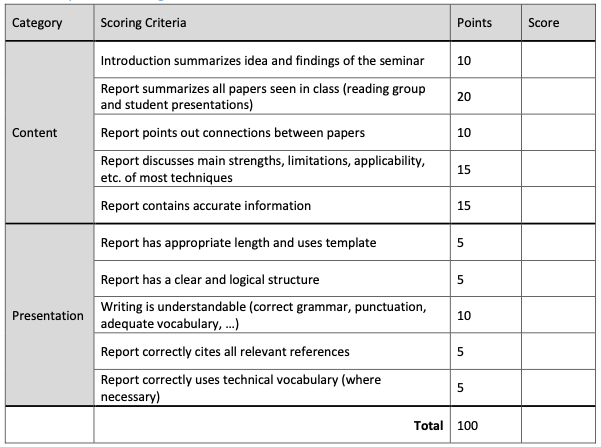
\includegraphics[scale = 0.72]{pictures/grading_scheme}\\

\newpage
\bibliography{finalReport}


\end{document}